\documentclass[conference]{IEEEtran}
\IEEEoverridecommandlockouts
\usepackage{cite}
\usepackage{amsmath,amssymb,amsfonts}
\usepackage{algorithmic}
\usepackage{graphicx}
\usepackage{textcomp}
\usepackage{xcolor}
\usepackage{hyperref}
\usepackage{tikz}
\usetikzlibrary{shapes.geometric, arrows, positioning}

\def\BibTeX{{\rm B\kern-.05em{\sc i\kern-.025em b}\kern-.08em
    T\kern-.1667em\lower.7ex\hbox{E}\kern-.125emX}}

\begin{document}

\title{TypeMaster AI: A Multimodal AI-Powered Typing Tutor for Personalized Skill Acquisition\\
}

\author{\IEEEauthorblockN{Jamadagni Gottipati}
\IEEEauthorblockA{\textit{Department of Computer Science and Engineering} \\
\textit{DVR \& Dr. HS MIC College of Technology}\\
Kanchikacherla, Andhra Pradesh, India \\
gottipatijamadagni@mictech.edu.in}
}

\maketitle

\begin{abstract}
Proficiency in touch typing remains a critical competency in the digital era, yet traditional typing tutors often rely on repetitive, static content that fails to maintain user engagement. This paper introduces TypeMaster AI, an advanced multimodal typing tutor that leverages Large Language Models (LLMs) to provide personalized and interactive learning experiences. By integrating the Gemini 2.0 API and OpenRouter, the system offers dynamic lesson generation based on user-defined topics, real-time grammar correction for custom inputs, and an immersive ``Melody Typing'' mode featuring predefined classical and contemporary music. Unlike standard tutors, this system utilizes high-performance browser APIs and concurrent React rendering to minimize input latency. The application is deployed and accessible at: \url{https://learn-key-board-you-like.vercel.app/}.
\end{abstract}

\begin{IEEEkeywords}
Typing Tutor, Multimodal AI, Large Language Models, Gemini API, OpenRouter, Web Audio API, React.js, Human-Computer Interaction.
\end{IEEEkeywords}

\section{Introduction}
Touch typing is a fundamental requirement for productivity in the modern digital landscape. Despite its importance, the pedagogical approach to typing has historically relied on static, unengaging corpora. TypeMaster AI revolutionizes this by treating typing as a multimodal, interactive experience powered by state-of-the-art Generative AI. By enabling users to practice using topics they are genuinely interested in---ranging from technical code snippets to creative prose---we bridge the gap between skill acquisition and user engagement.

\section{System Architecture and Implementation}
TypeMaster AI is built on a modular, decoupled architecture designed to handle high-frequency user inputs while maintaining a responsive UI.

\begin{figure}[h]
\centering
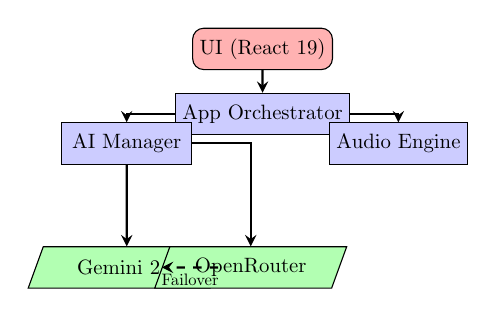
\begin{tikzpicture}[node distance=1.1cm, every node/.style={scale=0.75}]
\tikzstyle{startstop} = [rectangle, rounded corners, minimum width=2.2cm, minimum height=0.7cm,text centered, draw=black, fill=red!30]
\tikzstyle{process} = [rectangle, minimum width=2.2cm, minimum height=0.7cm, text centered, draw=black, fill=blue!20]
\tikzstyle{io} = [trapezium, trapezium left angle=70, trapezium right angle=110, minimum width=2.2cm, minimum height=0.7cm, text centered, draw=black, fill=green!30]
\tikzstyle{arrow} = [thick,->,>=stealth]

\node (ui) [startstop] {UI (React 19)};
\node (orchestrator) [process, below of=ui] {App Orchestrator};
\node (ai) [process, left of=orchestrator, xshift=-1.2cm, yshift=-0.5cm] {AI Manager};
\node (audio) [process, right of=orchestrator, xshift=1.2cm, yshift=-0.5cm] {Audio Engine};
\node (gemini) [io, below of=ai, yshift=-1.0cm] {Gemini 2.0};
\node (or) [io, right of=gemini, xshift=1.0cm] {OpenRouter};

\draw [arrow] (ui) -- (orchestrator);
\draw [arrow, ->] (orchestrator) -| (ai);
\draw [arrow, ->] (orchestrator) -| (audio);
\draw [arrow, ->] (ai) -- (gemini);
\draw [arrow, ->] (ai) -| (or);
\draw [arrow, dashed] (gemini) -- node[anchor=north, scale=0.8] {Failover} (or);

\end{tikzpicture}
\caption{System Architecture of TypeMaster AI demonstrating the dual-API failover strategy.}
\end{figure}

\subsection{Concurrent UI and State Persistence}
The application utilizes \textbf{React 19}'s concurrent rendering features to ensure that the typing state (tracked via \textit{useState} and \textit{useRef}) remains isolated from expensive UI re-renders. We specifically leverage \textbf{useCallback} hooks for the keyboard listener to prevent event-handler drift during high-speed typing sessions ($>100$ WPM). Application state, including user progress and search history, is persisted via a specialized \textit{LocalHistoryService} using the browser's \textit{localStorage} API.

\subsection{Real-time Auditory Synthesis}
To provide the ``Melody Typing'' experience, we developed a custom \textbf{Audio Service} based on the \textbf{Web Audio API}. Instead of pre-recorded samples which suffer from playback latency and memory overhead, we utilize an \textit{AudioContext} to dynamically create \textit{OscillatorNode} and \textit{GainNode} instances. Each keystroke triggers a frequency-modulated sine wave corresponding to a specific note in a musical sequence. This synthesis approach ensures zero-latency feedback, which is critical for maintaining the user's typing rhythm.

\section{AI Layer and LLM Orchestration}
The intelligence of TypeMaster AI is centered around a dual-path LLM orchestration layer.

\subsection{OpenRouter Failover and Rate-Limiting Protection}
As illustrated in Fig. 1, we implemented a sophisticated failover gateway. While the primary system targets the \textbf{Gemini 2.0 API} directly, production environments often encounter strict rate limits (RPM/TPM) or regional availability issues. We utilize \textbf{OpenRouter} as an abstraction layer to solve these challenges. 
By integrating OpenRouter, we ensure:
\begin{itemize}
    \item \textbf{High Availability:} If the primary Gemini key reaches its quota, the orchestrator automatically routes traffic through OpenRouter's distributed pool.
    \item \textbf{Latency Optimization:} OpenRouter provides edge-caching for similar generation requests, significantly reducing time-to-first-token (TTFT) for common lesson topics.
\end{itemize}

\subsection{Multimodal Input Processing}
The AI Manager handles more than just text. We leverage Gemini's multimodal capabilities to extract lessons from uploaded PDF and image files. The system uses a specialized prompt to ensure the output is returned as raw, typable text, stripping away metadata or conversational filler that typically accompanies LLM responses.

\section{Gamified Learning and User Feedback}
The immersive feedback loop is the core innovation of the product. By mapping character accuracy to musical harmony, we create a sensory-rich learning environment. The predefined library includes 50+ songs across classical and pop genres. Incorrect keystrokes trigger a discordant low-pass filtered sound, providing immediate negative reinforcement that encourages focus on accuracy over pure speed.

\section{Conclusion}
TypeMaster AI demonstrates that the synergy of modern web technologies (React, Web Audio API) and LLM orchestration (Gemini, OpenRouter) can transform a legacy educational task into an engaging, multimodal experience. By solving technical hurdles like input latency and API reliability, the system provides a robust platform for personalized skill acquisition. Future versions will integrate more complex multimodal interactions, such as live speech-to-typing drills. 

The production deployment is live at: \url{https://learn-key-board-you-like.vercel.app/}.

\section{References}
\begin{enumerate}
    \item J. S. Brown, ``Learning in the Digital Age,'' \textit{The Digital Media and Learning Series}, MIT Press, 2012.
    \item Google Research, ``Gemini: A Family of Highly Capable Multimodal Models,'' \textit{Technical Report}, 2023.
    \item R. S. Mayer, ``The Cambridge Handbook of Multimedia Learning,'' \textit{Cambridge University Press}, 2014.
    \item W3C, ``Web Audio API Specification,'' 2021. [Online]. Available: \url{https://www.w3.org/TR/webaudio/}
    \item Facebook Open Source, ``React 19 Documentation: Concurrent Rendering and Hooks,'' 2024.
\end{enumerate}

\end{document}

